\chapter{Regresión lineal}
\labch{regresion-lineal}

% Notación: \SSx, \SSy, \SSxy, \SSE y \SE están definidas en main.tex.

\begin{ideanote}
Cuando dos cosas se mueven juntas —el tamaño de un departamento y su arriendo, por ejemplo— nos gustaría resumir esa relación con algo simple, como una recta. ¿Cuál es la \emph{mejor} recta, y cuándo vale la pena usarla en vez de quedarnos con el promedio?
\end{ideanote}

\section{Introducción}
\labsec{regresion-introduccion}

Tenemos una base de datos con arriendos de departamentos en Santiago. De cada uno sabemos varias cosas, pero quedémonos con dos: su superficie útil (en metros cuadrados) y su arriendo mensual (en pesos). La pregunta es de las más cotidianas que hay: si me dicen que un departamento tiene \qty{50}{\meter\squared}, ¿cuánto esperaría pagar de arriendo?

Uno intuye que mientras más grande el departamento, más caro el arriendo. Esa es la \emph{señal}. Pero también sabemos que dos departamentos de la misma superficie pueden costar distinto: uno está mejor ubicado, otro más nuevo, otro tiene estacionamiento. Eso es el \emph{ruido}. Estamos, otra vez, en la historia de señal contra ruido del \nrefsec{senal-ruido}, sólo que ahora la señal no es un número fijo, sino que \emph{depende} de otra variable.

\begin{pausa}
Antes de seguir: si tuviera que resumir la relación entre superficie y arriendo con una sola figura geométrica, ¿cuál usaría? ¿Y por qué una recta y no, digamos, una curva?
\end{pausa}

Lo más simple que podemos proponer es que la señal es una \emph{recta}: que el arriendo esperado sube de manera constante con cada metro cuadrado extra. No es la única opción ni siempre la mejor, pero es la primera que conviene probar, y muchas veces alcanza. A esto se le llama \emph{regresión lineal}: ajustar una recta a una nube de puntos.

\section{¿Mejor que el promedio?}
\labsec{mejor-que-promedio}

Antes de buscar la recta, preguntémonos algo más básico: ¿para qué la queremos? La respuesta es \emph{para predecir mejor}. Y \enquote{mejor} sólo tiene sentido comparado con algo. Ese algo es el promedio.

Imaginemos que no nos dejan mirar la superficie. Sólo tenemos los arriendos. Si nos piden adivinar el arriendo de un departamento cualquiera, la mejor apuesta que tenemos es el promedio de todos los arriendos, \(\mean{y}\).\sidenote{de hecho, el promedio es justamente el número que minimiza la suma de los cuadrados de las diferencias; lo vimos al hablar de la esperanza como centro de masa} Por supuesto, casi siempre nos vamos a equivocar. A la diferencia entre el arriendo real y nuestra predicción la llamamos \emph{residuo}, y una forma de medir cuánto nos equivocamos en total es sumar todos esos residuos al cuadrado.\sidenote{los elevamos al cuadrado por la misma razón de siempre: para que no se cancelen los positivos con los negativos, y para castigar más los errores grandes}

Tomemos seis departamentos para verlo con números amables. Sus superficies útiles y arriendos (en miles de pesos) son:

\begin{center}
\begin{tabular}{rSSSSSS}
\toprule
Superficie \(x\) (\unit{\meter\squared}) & 20 & 30 & 40 & 50 & 60 & 70 \\
Arriendo \(y\) (miles \$) & 230 & 250 & 390 & 480 & 520 & 680 \\
\bottomrule
\end{tabular}
\end{center}

El promedio de los arriendos es \(\mean{y}=\num{425}\) (miles de pesos). Si predecimos \(\num{425}\) para todos, los residuos son las distancias verticales de cada punto a esa recta horizontal.

\begin{center}
\begin{tikzpicture}
  \begin{axis}[
    width=\linewidth, height=6cm,
    axis lines=left,
    xlabel={Superficie útil (\unit{\meter\squared})},
    ylabel={Arriendo (miles \$)},
    xmin=12, xmax=78, ymin=150, ymax=720,
    xtick={20,30,40,50,60,70},
    clip=false,
  ]
    \addplot[DiceRed, thin] coordinates {(20,230) (20,425)};
    \addplot[DiceRed, thin] coordinates {(30,250) (30,425)};
    \addplot[DiceRed, thin] coordinates {(40,390) (40,425)};
    \addplot[DiceRed, thin] coordinates {(50,480) (50,425)};
    \addplot[DiceRed, thin] coordinates {(60,520) (60,425)};
    \addplot[DiceRed, thin] coordinates {(70,680) (70,425)};
    \addplot[black, thick, domain=12:78] {425};
    \addplot[only marks, mark=*, DiceBlue!80!black] coordinates
      {(20,230) (30,250) (40,390) (50,480) (60,520) (70,680)};
    \node[anchor=south west, font=\small] at (axis cs:12,425) {\(\mean{y}=\num{425}\)};
  \end{axis}
\end{tikzpicture}
\end{center}

La suma de esos residuos al cuadrado resulta ser \(\num{146950}\). Llamemos a este número \(\SSy\): es cuánto nos equivocamos usando \emph{sólo} la información de \(y\).

Ahora miremos la superficie y ajustemos una recta inclinada (en un momento veremos de dónde sale). Los residuos pasan a ser las distancias verticales a esa nueva recta:

\begin{center}
\begin{tikzpicture}
  \begin{axis}[
    width=\linewidth, height=6cm,
    axis lines=left,
    xlabel={Superficie útil (\unit{\meter\squared})},
    ylabel={Arriendo (miles \$)},
    xmin=12, xmax=78, ymin=150, ymax=720,
    xtick={20,30,40,50,60,70},
    clip=false,
  ]
    \addplot[DiceRed, thin] coordinates {(20,230) (20,200)};
    \addplot[DiceRed, thin] coordinates {(30,250) (30,290)};
    \addplot[DiceRed, thin] coordinates {(40,390) (40,380)};
    \addplot[DiceRed, thin] coordinates {(50,480) (50,470)};
    \addplot[DiceRed, thin] coordinates {(60,520) (60,560)};
    \addplot[DiceRed, thin] coordinates {(70,680) (70,650)};
    \addplot[MidnightBlue, thick, domain=14:76] {20+9*x};
    \addplot[only marks, mark=*, DiceBlue!80!black] coordinates
      {(20,230) (30,250) (40,390) (50,480) (60,520) (70,680)};
    \node[anchor=north west, font=\small, MidnightBlue] at (axis cs:50,470) {\(\estim{y}=20+9x\)};
  \end{axis}
\end{tikzpicture}
\end{center}

Si sumamos \emph{estos} residuos al cuadrado obtenemos \(\num{5200}\). Llamémoslo \(\SSE\), la suma de cuadrados de los residuos de la recta. Y aquí está lo importante:
\[\underbrace{\num{5200}}_{\SSE\text{ (con }x\text{)}} \;<\; \underbrace{\num{146950}}_{\SSy\text{ (sólo }y\text{)}}.\]

Considerar la superficie hizo que nos equivocáramos mucho menos. Esa es, en el fondo, toda la justificación de la regresión: \emph{una recta sirve cuando la suma de cuadrados de los residuos es menor al considerar ambas variables que al considerar sólo \(y\).} Si la recta no lograra bajar esa suma, no estaríamos ganando nada y daría lo mismo usar el promedio.

\section{La recta de mínimos cuadrados}
\labsec{minimos-cuadrados}

Ya tenemos el criterio: queremos la recta que haga \(\SSE\) lo más chico posible. De ahí el nombre \emph{mínimos cuadrados}. Pero antes de buscarla, ordenemos la notación, porque vamos a necesitar tres cantidades una y otra vez.

\formal
Definimos las \emph{sumas de cuadrados}
\[\SSx = \sum (x_i-\mean{x})^2, \qquad \SSy = \sum (y_i-\mean{y})^2, \qquad \SSxy = \sum (x_i-\mean{x})(y_i-\mean{y}).\]
\informal

\(\SSx\) y \(\SSy\) miden cuánto se dispersan \(x\) e \(y\) por su cuenta; \(\SSxy\) mide cómo se mueven \emph{juntas} (es el numerador de la covarianza).

\marginnote{Una advertencia de notación. En muchos textos en español estas cantidades se escriben \(S_{xx}\), \(S_{yy}\), \(S_{xy}\). El problema es que \(S_{xx}\) se parece demasiado a \(s_x\), la desviación estándar muestral, y es fácil confundirlas (de hecho \(\SSx=(n-1)s_x^2\), así que ni siquiera son lo mismo). Por eso en este texto preferimos \(\SSx\), \(\SSy\), \(\SSxy\).}

Ahora sí, busquemos la recta. Hay que decir algo sobre qué representa. El arriendo de un departamento de superficie \(x\) no está \emph{determinado} por \(x\): hay ruido. Lo que proponemos es que la parte sistemática —la señal— es una recta. Es decir, que el arriendo esperado es \(a + b x\), donde \(a\) es el punto de partida (el intercepto) y \(b\) es cuánto sube el arriendo por cada metro cuadrado extra (la pendiente).

\begin{pausa}
\(a\) y \(b\) son números que describen a \emph{toda} la población de departamentos, pero nosotros sólo tenemos una muestra. ¿Le suena esta situación de algún capítulo anterior?
\end{pausa}

Exacto: \(a\) y \(b\) son parámetros poblacionales que no conocemos, igual que \(\mu\) o \(\sigma\) en su momento. Lo que calculamos a partir de la muestra son \emph{estimadores}, y por eso, para ser rigurosos, deberíamos escribirlos con sombrero: \(\estim{a}\) y \(\estim{b}\). La predicción que entrega la recta también es un estimador, el del arriendo esperado, y se escribe \(\estim{y}\):
\[\estim{y} = \estim{a} + \estim{b}\,x.\]
Para no llenar todo de sombreros, muchas veces escribiremos simplemente \(a + bx\); pero tengamos siempre presente que \(a\) y \(b\) son estimadores que cambian si cambia la muestra.

\formal
Encontrar la mejor recta es minimizar \[\SSE(a,b) = \sum \left(y_i - a - b x_i\right)^2\] sobre todos los \(a\) y \(b\) posibles. Como es una función de dos variables, derivamos respecto de cada una y la igualamos a cero. Respecto de \(a\),
\[\frac{\partial \,\SSE}{\partial a} = -2\sum\left(y_i - a - b x_i\right) = 0 \;\Longrightarrow\; \mean{y} = \estim{a} + \estim{b}\,\mean{x},\]
es decir, la recta pasa por el punto promedio \((\mean{x}, \mean{y})\). De ahí despejamos el intercepto, \(\estim{a} = \mean{y} - \estim{b}\,\mean{x}\). Respecto de \(b\), tras un poco de álgebra que dejaremos como ejercicio al lector, se llega a
\[\estim{b} = \frac{\SSxy}{\SSx}.\]
\informal

Vale la pena mirar esas dos fórmulas con cariño. La pendiente \(\estim{b}=\SSxy/\SSx\) es cómo se mueven juntas \(x\) e \(y\), dividido por cuánto se mueve \(x\) sola. Y el intercepto \(\estim{a}=\mean{y}-\estim{b}\,\mean{x}\) no es más que la condición de que la recta pase por el centro de la nube. Dos fórmulas, nada más, y con eso tenemos la mejor recta posible.

\subsection{El ejemplo, ahora con números}

Volvamos a nuestros seis departamentos. Conviene calcular primero las medias: \(\mean{x}=45\) y \(\mean{y}=425\). Con eso armamos la tabla de desviaciones:

\begin{center}
\begin{tabular}{SSSSS}
\toprule
{\(x-\mean{x}\)} & {\(y-\mean{y}\)} & {\((x-\mean{x})^2\)} & {\((y-\mean{y})^2\)} & {\((x-\mean{x})(y-\mean{y})\)} \\
\midrule
-25 & -195 & 625 & 38025 & 4875 \\
-15 & -175 & 225 & 30625 & 2625 \\
-5  & -35  & 25  & 1225  & 175  \\
5   & 55   & 25  & 3025  & 275  \\
15  & 95   & 225 & 9025  & 1425 \\
25  & 255  & 625 & 65025 & 6375 \\
\midrule
{} & {} & 1750 & 146950 & 15750 \\
\bottomrule
\end{tabular}
\end{center}

Las tres sumas de la última fila son justamente \(\SSx=\num{1750}\), \(\SSy=\num{146950}\) y \(\SSxy=\num{15750}\). Entonces
\[\estim{b} = \frac{\SSxy}{\SSx} = \frac{\num{15750}}{\num{1750}} = 9, \qquad \estim{a} = \mean{y} - \estim{b}\,\mean{x} = 425 - 9\cdot 45 = 20.\]
La recta es \(\estim{y} = 20 + 9x\) (en miles de pesos), que es exactamente la que dibujamos antes. Cada metro cuadrado extra agrega unos \(9\) mil pesos al arriendo, y el intercepto es \(20\) mil. Por ejemplo, para un departamento de \qty{55}{\meter\squared} predeciríamos \[\estim{y} = 20 + 9\cdot 55 = 515\] mil pesos.

\section{¿Qué tan buena es la recta?}
\labsec{bondad-ajuste}

Ya sabemos que la recta baja la suma de cuadrados de \(\num{146950}\) a \(\num{5200}\). Podemos convertir esa mejora en un número que vaya de \(0\) a \(1\) y se interprete fácil. La idea es preguntarse \emph{qué fracción} de la dispersión original de \(y\) logramos explicar con la recta.

\formal
La dispersión total se descompone en dos partes,
\[\underbrace{\SSy}_{\text{total}} = \underbrace{\estim{b}\,\SSxy}_{\text{explicada por la recta}} + \underbrace{\SSE}_{\text{residual}},\]
y definimos el \emph{coeficiente de determinación} como la fracción explicada,
\[r^2 = \frac{\text{explicada}}{\text{total}} = 1 - \frac{\SSE}{\SSy}.\]
\informal

De paso, esa descomposición nos da una forma corta de calcular el residual sin pasar por cada predicción: como \(\estim{b}=\SSxy/\SSx\), \[\SSE = \SSy - \estim{b}\,\SSxy = \SSy - \frac{\SSxy^2}{\SSx}.\]

En nuestro ejemplo, \[r^2 = 1 - \frac{\num{5200}}{\num{146950}} = \num{0,965},\] es decir, la superficie explica cerca del \qty{96}{\percent} de la variación en los arriendos de estos seis departamentos. El resto, ese \qty{4}{\percent}, es el ruido que la recta no captura. Un \(r^2\) cercano a \(1\) dice que los puntos se pegan a la recta; uno cercano a \(0\), que la recta no sirve de mucho.

La raíz de \(r^2\), con el signo de la pendiente, es el \emph{coeficiente de correlación}, \[r = \frac{\SSxy}{\sqrt{\SSx\,\SSy}},\] que en nuestro ejemplo vale \(r\approx\num{0,98}\). La correlación nos muestra otra cara de la pendiente: si la escribimos en términos de las desviaciones muestrales de \(x\) e \(y\), \[\estim{b} = r\,\frac{s_y}{s_x},\] vemos que la pendiente es la correlación reescalada por cuánto se dispersa \(y\) frente a \(x\).

Por supuesto, seis departamentos elegidos para que salieran bonitos son una cosa, y la realidad es otra. La \reffig{arriendos-real} muestra los \num{1684} departamentos de verdad de la base de datos.

\begin{figure}[h]
\centering
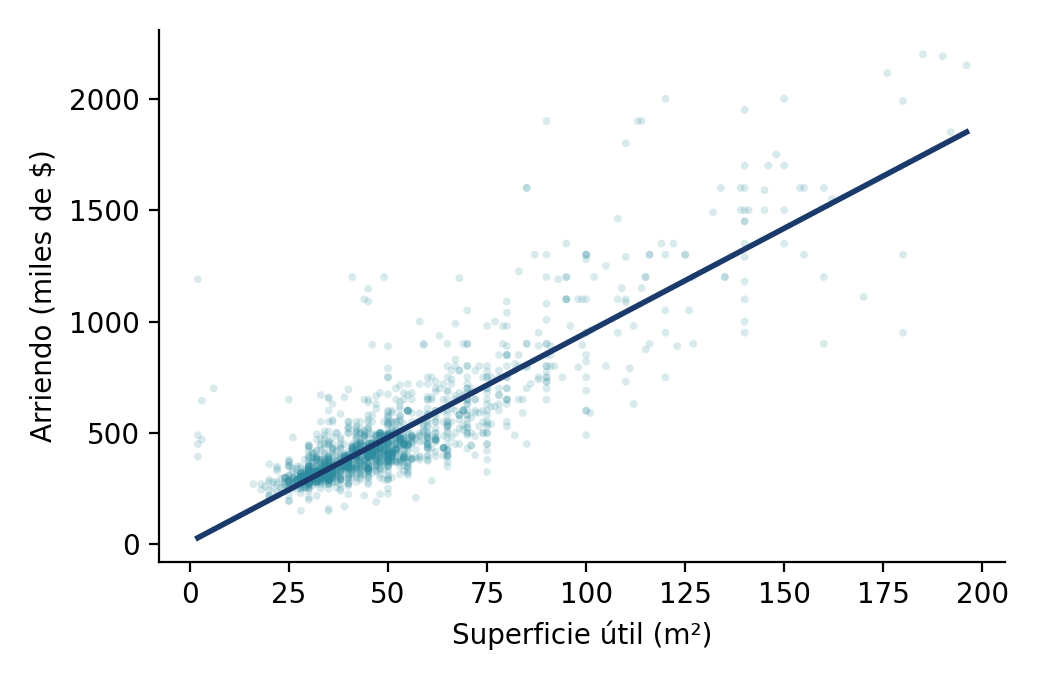
\includegraphics[width=\linewidth]{images/arriendos_regresion.png}
\caption{Arriendo contra superficie útil para \num{1684} departamentos, con la recta de mínimos cuadrados.}
\labfig{arriendos-real}
\end{figure}

La nube es mucho más desordenada, como era de esperar, pero la señal lineal está clarísima. Los mismos cálculos sobre los datos reales dan una pendiente de unos \(\num{9386}\) pesos por metro cuadrado y un intercepto cercano a \(\num{10887}\) pesos, con \[r^2 \approx \num{0,74}.\] O sea, la superficie útil explica por sí sola un \qty{74}{\percent} de la variación de los arriendos. Nada mal para una sola variable: el \qty{26}{\percent} restante es todo lo demás —ubicación, antigüedad, estado— que no estamos mirando.

\section{¿La pendiente dice algo de verdad?}
\labsec{prueba-pendiente}

Queda una pregunta. Nuestra pendiente \(\estim{b}\) salió de una muestra. Si la relación entre superficie y arriendo en realidad no existiera —si la verdadera pendiente poblacional \(b\) fuera \(0\)— igual podríamos sacar, por puro azar de la muestra, una pendiente estimada distinta de cero. ¿Cómo distinguimos una pendiente \enquote{real} de una que es puro ruido muestral?

Esto es, palabra por palabra, una prueba de hipótesis como las del capítulo anterior. La hipótesis nula es que no hay relación lineal,
\[H_0: b = 0, \qquad H_a: b \neq 0,\]
y la lógica es la misma de siempre: comparamos la pendiente estimada con su propio error estándar. Si \(\estim{b}\) es grande comparada con cuánto suele variar de muestra en muestra, creeremos que la relación es real.

\formal
Primero estimamos cuánto ruido quedó, con la \emph{varianza residual} \(s_e^2\) (a veces llamada \(\mathrm{MSE}\)), y con ella el error estándar de la pendiente. El estadístico de prueba es
\[s_e^2 = \frac{\SSE}{n-2}, \qquad \SE(\estim{b}) = \sqrt{\frac{s_e^2}{\SSx}}, \qquad T = \frac{\estim{b}}{\SE(\estim{b})},\]
y bajo \(H_0\) sigue una distribución \(t\) de Student con \(n-2\) grados de libertad.
\informal

No profundizaremos más que esto. Lo importante es la idea: la pendiente vale como evidencia de una relación cuando es grande \emph{en relación a su error}. En nuestros seis departamentos, \(s_e^2=\num{5200}/4=\num{1300}\), de donde \(\SE(\estim{b})=\sqrt{\num{1300}/\num{1750}}\approx\num{0,86}\) y
\[T = \frac{9}{\num{0,86}} \approx \num{10,4},\]
con \(4\) grados de libertad: mucho más grande que cualquier valor crítico razonable, así que rechazamos \(H_0\). En los datos reales el estadístico es todavía mayor (del orden de \(70\)): que el arriendo suba con la superficie no es casualidad de la muestra.

Y con eso cerramos el recorrido. Partimos preguntándonos cuánto pagar por un departamento de cierto tamaño y terminamos con una recta que lo predice, una medida de qué tan bien lo hace, y una prueba de que la relación es real. La regresión lineal es la puerta de entrada a algo mucho más grande —se pueden meter varias variables a la vez, curvas en vez de rectas, y un largo etcétera— pero la idea de fondo no cambia: buscar la señal que mejor explica los datos y, sobre todo, saber medir cuánto del ruido quedó afuera.

\section{Resumen}
\labsec{regresion-resumen}

Para tener todo a mano, juntamos aquí las fórmulas del capítulo. Recordemos que \(a\) y \(b\) son estimadores —van con sombrero— y que \(n\) es el tamaño de la muestra.

\formal
\emph{Sumas de cuadrados.}
\[\SSx = \sum (x_i-\mean{x})^2, \qquad \SSy = \sum (y_i-\mean{y})^2, \qquad \SSxy = \sum (x_i-\mean{x})(y_i-\mean{y}).\]

\emph{Recta de mínimos cuadrados.}
\[\estim{b} = \frac{\SSxy}{\SSx} = r\,\frac{s_y}{s_x}, \qquad \estim{a} = \mean{y} - \estim{b}\,\mean{x}, \qquad \estim{y} = \estim{a} + \estim{b}\,x.\]

\emph{Bondad del ajuste.}
\[r = \frac{\SSxy}{\sqrt{\SSx\,\SSy}}, \qquad \SSE = \SSy - \frac{\SSxy^2}{\SSx} = \SSy - \estim{b}\,\SSxy, \qquad r^2 = \frac{\SSxy^2}{\SSx\,\SSy} = 1 - \frac{\SSE}{\SSy}.\]

\emph{Inferencia sobre la pendiente} (\(H_0: b=0\)).
\[s_e^2 = \frac{\SSE}{n-2}, \qquad \SE(\estim{b}) = \sqrt{\frac{s_e^2}{\SSx}}, \qquad T = \frac{\estim{b}}{\SE(\estim{b})} \sim \Td_{\,n-2}.\]
\informal
